\documentclass[conference]{IEEEtran}
\IEEEoverridecommandlockouts

\usepackage{cite}
\usepackage{amsmath,amssymb,amsfonts}
\usepackage{graphicx}
\usepackage{textcomp}
\usepackage{booktabs}
\usepackage{hyperref}
\hypersetup{colorlinks=true,citecolor=blue,linkcolor=red,urlcolor=blue}
\usepackage{url}
\usepackage{xurl}
\usepackage[table]{xcolor}
\usepackage{tabularx}
\usepackage{multirow}
\usepackage{enumitem}
\setlist{leftmargin=*,itemsep=1pt,topsep=2pt}
\Urlmuskip=0mu plus 1mu

\newcommand{\DC}{\textsc{DeepCTI}}
\newcommand{\Bel}[1]{\textsf{#1}}

\begin{document}

\title{DeepCTI: Evidence State Control for\\Threat Mitigation Decisions}

\author{
\IEEEauthorblockN{Anonymous Author(s)}
\IEEEauthorblockA{Anonymous Institution}
}

\maketitle

\begin{abstract}
Cyber threat intelligence (CTI) states which software versions are vulnerable, but deciding whether a
particular host is affected, and whether an agent may change it, depends on local evidence that can be
missing, noisy, stale or adversarial. We argue that LLM-assisted mitigation should be governed by an
explicit evidence state, not by the model's reasoning trace. \DC{} keeps a provenance-tracked
four-valued (Belnap) state over VEX-relevant atoms, counts support in independence groups of trusted
sources, decides with a deterministic VEX table that abstains on missing or conflicting evidence,
acquires evidence by value of information, admits LLM-extracted facts only after span verification, and
authorizes disruptive tools through Cedar policies that require independent trusted support. We
evaluate on two new live-fixture benchmarks with sealed labels: D1 (906 Debian hosts) and D7 (822 hosts
spanning Ubuntu, PyPI, Maven and vendor software). Baselines include scanners, a tracker lookup, direct
prompting and ReAct agents (ours and Inspect AI's), run with up to ten open models from 4B to 128B parameters
across four pre-registered rounds (about 270k test and calibration episodes). Without a vulnerability feed, \DC{} lowers
decision loss relative to ReAct by 1.58 (D1) and 0.88 (D7) with no dangerous errors. On vendor software,
where versions exist only in text, verified LLM extraction lowers loss by 0.21 relative to an LLM-free
controller. Learn-then-Test
releases abstentions at realised risk below 2\%, raising coverage from 0.31 to 0.50--0.91.
Evidence-gated authorization removes the 5--6\% of episodes in which an unmodified ReAct agent takes an
unauthorized disruptive action. We also report where the design fails: a restart-blind controller
(repaired by instance-aware evidence, loss 9.67 to 0.42), conservative trust estimation that discards
useful scanners, and injection attacks too weak to discriminate defences.
\end{abstract}

\begin{IEEEkeywords}
Cyber threat intelligence, vulnerability management, VEX, LLM agents, evidence state, authorization
\end{IEEEkeywords}

%==============================================================================
\section{Introduction}

Cyber threat intelligence (CTI) describes vulnerabilities, affected products and possible mitigations.
Acting on it requires local facts: whether the product is installed, which version is on disk and which is
running, whether a backport already fixed the flaw, and whether a vulnerable feature is enabled. Patch
management studies show that remediation also depends on testing, coordination and service
availability~\cite{dissanayake2022automation,jenkins2024patching,souppaya2022patchmanagement}. The
output that operators need is a VEX statement (\emph{affected}, \emph{not affected} with a
justification, \emph{fixed}, or \emph{under investigation})~\cite{oasis2022csaf}, and, where a change is
warranted, an authorized remediation.

Large language model (LLM) agents that interleave reasoning with tool
calls~\cite{yao2023react,schick2023toolformer} can gather this evidence, and LocalIntel shows that
combining global CTI with organization-specific context helps~\cite{mitra2024localintel}. Our
measurements, however, show that such agents fail in a specific and costly way: they \emph{miss}
vulnerabilities. A ReAct agent misses 34--49\% of affected Debian hosts in our benchmark, and its loss varies
fifteenfold across models. They also take disruptive actions they were not authorized to
take, even without any attacker. Both failures stem from the same design choice: the agent's beliefs
about the host live only in its context window, without provenance, trust or freshness.

We argue that CTI-driven mitigation should be governed by an explicit \emph{evidence state}: a record of
which trusted, independent, fresh observations support or refute each decision-relevant fact. The state
determines the decision and gates every action, and the language model is confined to roles where it can
be checked. This leads to two research questions.

\textbf{RQ-1:} Which evidence state, decision rule and acquisition strategy yield correct, abstaining-when-unsure
VEX decisions as observations arrive, conflict and go stale?

\textbf{RQ-2:} How should mitigation judgments be connected to authorization so that investigative and
disruptive actions remain within policy, including when some sources are adversarial?

\textbf{Contributions.}
\begin{itemize}
\item \textbf{Design.} \DC{} combines several mechanisms (\S\ref{sec:design}):
  \begin{itemize}
  \item a provenance-tracked Belnap evidence state with trust classes, independence groups and
    freshness windows;
  \item a deterministic VEX decision table;
  \item value-of-information (EC$^2$) acquisition;
  \item span-verified LLM extraction;
  \item Learn-then-Test release of hint-based decisions;
  \item evidence-conditioned Cedar authorization with a fragment linter that guarantees a $k$-of-$n$
    corroboration property.
  \end{itemize}
\item \textbf{Benchmarks.} D1 and D7 are live-fixture benchmarks: root file systems built from official
  base images, with package databases, version files, jar metadata and real scanner reports. Labels come
  from authoritative trackers, and test splits are sealed. They are extended with drift (D2, X5) and adversarial (D3) episodes (\S\ref{sec:eval}).
\item \textbf{Pre-registered evaluation.} We test 19 hypotheses over four tagged pre-registration rounds,
  ten open models and a third-party baseline, reporting failed hypotheses and post-hoc corrections
  (\S\ref{sec:results}).
\item \textbf{Findings.} We characterize what the LLM contributes in such a system: little where evidence is
  structured, and a measurable gain where it is not. We identify two failure modes, restart blindness and
  over-conservative trust, and we evaluate repairs for both.
\end{itemize}

%==============================================================================
\section{Related Work}

\textbf{CTI and mitigation.} CTIBench, AthenaBench, CTIConnect and ExCyTIn-Bench evaluate CTI knowledge,
mitigation mapping, retrieval over CTI sources and interactive
investigation~\cite{alam2024ctibench,alam2025athenabench,cheng2025cticonnect,wu2025excytin}. None asks
whether a specific host is affected. LocalIntel contextualizes CTI with organizational
knowledge~\cite{mitra2024localintel}, and TrustOps argues for evidence-grounded defence under missing,
conflicting and stale evidence~\cite{malamas2026trustops}. Patch-management studies document delays,
testing needs and failures of security
patches~\cite{dissanayake2022automation,dissanayake2022delays,li2017securitypatches,jenkins2024patching},
and NIST guidance covers configuration monitoring~\cite{johnson2011configuration,dempsey2011monitoring}.
\DC{} turns these requirements into a decision procedure with measurable loss.

\textbf{Retrieval, reasoning and verification.} RAG and its corrective and reflective variants ground
generation in retrieved text~\cite{lewis2020rag,asai2024selfrag,yan2024crag,he2024covrag}. Freshness and
conflict-aware retrieval address changing
knowledge~\cite{vu2024freshllms,ozer2025temporalconflict,nie2026evotrustrag}, and misleading context
degrades answers~\cite{hong2024gullible}. Memory systems such as MemGPT keep long-lived
context~\cite{packer2023memgpt}. In all of these, retrieved text informs a generated answer. In \DC{}, an
observation changes the decision only through a trusted source's verified fact, and untrusted text
remains a hint.

\textbf{Agent authorization.} Least privilege, complete mediation and attribute-based access control are
the classical
foundations~\cite{saltzer1975protection,hu2014abac,hu2019attributes}. Progent, AgentSpec, CaMeL and
DRIFT constrain agent tool use by privilege, runtime rules, data-flow separation or
isolation~\cite{shi2025progent,wang2026agentspec,debenedetti2025camel,li2025drift}, and
\cite{siu2026agentsecurity} formalizes action alignment and source authorization. Closest to our
corroboration rule are TMA-NM~\cite{louck2026tmanm} and certified multi-source
integrity~\cite{pandey2026certified}, which admit an action only with support from several independent
trusted principals or domains. \DC{} differs in three ways. Its evidence state is four-valued and
time-indexed. Its policies are standard Cedar~\cite{cutler2024cedar}, linted into a fragment for which the
guarantee holds. Its decision semantics are those of deployed VEX. AgentDojo, InjecAgent, ToolEmu and
R-Judge evaluate injection and risk
awareness~\cite{debenedetti2024agentdojo,zhan2024injecagent,ruan2024toolemu,yuan2024rjudge}; we follow
\cite{bhagwatkar2025injectionbenchmarks} in reporting the benign error rate next to attack success.

\textbf{Active acquisition and risk control.} EC$^2$ selects tests that separate decision regions at low
expected cost~\cite{golovin2010ec2,golovin2011adaptive}. Learn-then-Test (LTT) selects parameters of a
predictor with finite-sample risk control~\cite{angelopoulos2021ltt}, and \cite{wu2026safetostop} applies
LTT-style tests to decide when a clinical diagnosis agent may stop. VEX-Bench evaluates VEX status
prediction on source repositories~\cite{vexbench2026}. We combine both with a Belnap
state~\cite{belnap1977useful}, so that ``unknown'' and ``conflicting'' are first-class outcomes.

%==============================================================================
\section{DeepCTI}
\label{sec:design}

\begin{figure*}[t]
\centering
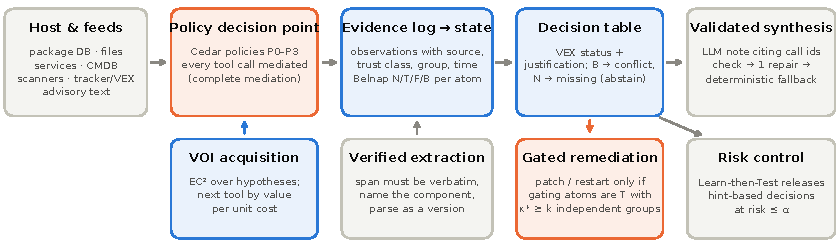
\includegraphics[width=\textwidth]{figs/fig_architecture.pdf}
\caption{\DC{} architecture. Every tool call passes the policy decision point. Tool outputs become
observations with source, trust class, independence group and time. The deterministic VEX table reads
the state, and the LLM proposes extractions (verified before entering the state), advisory hints and the
analyst note (validated). Disruptive tools need gating atoms supported by $\ge k$ independent trusted groups.}
\label{fig:architecture}
\end{figure*}

\subsection{Setting and threat model}

A case is a pair (host, CVE). The agent sees only the host name, release, CVE and component name, and it acts
through mediated tools:
\begin{itemize}
\item read tools: package query, file read, directory listing, service status, configuration read,
  language-package query, CMDB lookup, advisory fetch, tracker/VEX lookup;
\item medium-risk tools: scanner run, change approval request;
\item disruptive tools: patch, restart, feature disable.
\end{itemize}
Each tool has a cost: read tools cost 1, a scanner run 5, a patch 20 and a restart 15; the budget is 60.
Each \emph{source} carries a trust class (T/U) and an \emph{independence group}:
\begin{itemize}
\item \texttt{pkgdb}: the package database, and also the scanners, which read it;
\item \texttt{fs}: changelogs, configuration and version files;
\item \texttt{proc}: process view and banners;
\item \texttt{langdb}/\texttt{artifact}: language-package metadata and jar contents (D7);
\item \texttt{change}: approvals and rollback;
\item feeds (tracker and VEX), CMDB and advisories, each in its own group.
\end{itemize}
Trust is estimated on the development split. A source is trusted iff the Wilson 95\% upper bounds of its
false-positive and false-negative rates are both $\le 0.10$ with $n\ge 20$. Advisory text, CMDB notes and
anything an LLM compiles are untrusted. The attacker can inject arbitrary untrusted text, and can
compromise up to $m$ trusted groups so that they report forged values.

\subsection{Evidence state}

An observation is $(f, \pm, s, t, h)$: atom $f$, polarity, source $s$, time $t$ and content hash $h$. The
world atoms are \texttt{present}, \texttt{in\_affected\_range}, \texttt{fix\_applied} and
\texttt{vuln\_config\_enabled}. The change atoms are \texttt{change\_approved},
\texttt{rollback\_available} and \texttt{in\_maintenance\_window}. For each atom, the state takes the
latest \emph{fresh} observation of every trusted source. Freshness windows are $\Delta=12$ time units for
world atoms and $30$ for change atoms. The state then counts positive and negative support in distinct
independence groups:
\begin{equation}
\kappa^{\pm}_f = \bigl|\{\,g(s) : s\in\mathcal{T},\ \mathrm{last}_\Delta(s,f)=\pm\}\bigr|,
\end{equation}
where $\mathcal{T}$ is the set of trusted sources, $g(s)$ the group of $s$, and
$\mathrm{last}_\Delta(s,f)$ the polarity of the latest observation of $f$ by $s$ within the window.
The Belnap value is \Bel{T} if $\kappa^+_f>0=\kappa^-_f$, \Bel{F} in the converse case, \Bel{B} (both) if
both counts are positive, and \Bel{N} (none) otherwise~\cite{belnap1977useful}. Untrusted observations
never change a value; they are kept as hints. The log is append-only, and only tool executions (including the carried-over history of earlier ones)
write to it.

\subsection{Decision table}

The VEX decision is a pure function of the atom values, evaluated row by row:
\begin{itemize}
\item \texttt{present}=\Bel{F} gives \emph{not affected} (component not present).
\item \texttt{fix\_applied}=\Bel{T} gives \emph{fixed}.
\item \texttt{in\_affected\_range}=\Bel{F} gives \emph{not affected} (vulnerable code not present).
\item If the CVE has a configuration precondition, \texttt{vuln\_config\_enabled}=\Bel{F} gives
  \emph{not affected} (requires configuration).
\item Otherwise the decision is \emph{affected}.
\end{itemize}
A \Bel{B} on a consulted atom yields \emph{under investigation} (conflict). An \Bel{N} on an atom that
blocks every later row yields \emph{under investigation} (missing), together with the atoms whose
acquisition would decide the case.
Abstention is therefore explicit and explained, never a guess.

\textbf{Running example.} CVE-2024-6387 (regreSSHion) affects upstream OpenSSH 8.6--9.8. Consider a
Debian~12 host with \texttt{openssh-server} \texttt{1:9.2p1-2+deb12u3}. Its upstream version lies inside
the range, so a naive comparison says \emph{affected}, but this Debian revision is the tracker's fixed
version (a backport). \DC{} reads the installed version from the package database and the fixed version
from the tracker. It sets \texttt{present}=\Bel{T} and \texttt{fix\_applied}=\Bel{T}, and decides
\emph{fixed} after two calls. If the package was upgraded but \texttt{sshd} still runs the old build,
the decision changes. The instance-aware version below observes \texttt{running\_fix\_applied}=\Bel{F}
from the process view and decides \emph{affected}. A restart is then permitted only with an approved
change inside a maintenance window.

\textbf{Instance-aware evidence (v2.1).} Our first evaluation exposed a failure: a package upgraded on
disk while the old binary keeps running is reported \emph{fixed} from the package database. v2.1 adds the
atoms \texttt{running\_in\_affected\_range} and \texttt{running\_fix\_applied}, observed from the process
view. A component is in range if \emph{any} instance, on disk or running, is in range, and it is fixed only
if \emph{all} observed instances are fixed. Before deciding \emph{fixed} or \emph{not affected} (code not present),
acquisition must consult the process view.

\subsection{Acquisition}

Given priors over hypotheses (joint assignments of the atoms) estimated on the development split,
\DC{} chooses the next tool by EC$^2$: the expected weight of edges cut between hypotheses with different
decisions, per unit cost~\cite{golovin2010ec2}. It stops when every hypothesis consistent with the state
yields the same decision, or when the budget is exhausted. Ablations replace EC$^2$ with entropy-greedy,
a fixed checklist, random order, or an LLM choosing the next tool.

\subsection{Verified LLM extraction}

Where evidence is text (changelogs, release notes, banners, manifests), the LLM proposes facts of the form
(atom or version, value, verbatim span, call id). A verifier admits a fact only if:
\begin{itemize}
\item the span occurs verbatim in that call's output;
\item the span names the component, with the version as the first version token within 40 characters;
\item it comes from a grammar-sanctioned location: the changelog header line, a vendor version document,
  or a process line (for Debian/Ubuntu only the line naming the package build, since an upstream banner
  cannot establish a distribution revision);
\item it parses as a version of the ecosystem: dpkg semantics for Debian/Ubuntu, \texttt{univers} for
  PyPI, Maven and vendor versions.
\end{itemize}
An admitted fact becomes an observation of the underlying (trusted) source. Advisory text that the LLM
compiles into version ranges remains untrusted, so it yields hints only.

\subsection{Risk-controlled release}

When no trusted source decides a case, \DC{} abstains. In that case the hints (an LLM-compiled advisory
range applied to verified versions) often point to a decision. We release hint-based decisions with LTT~\cite{angelopoulos2021ltt}. The score of an abstention is
the smallest support margin (trusted plus hint support for the hinted value, minus support against it)
over the atoms the decision needs. Thresholds are tested from strict to loose, in fixed sequence, with
Hoeffding--Bentkus $p$-values. The selected threshold satisfies $\Pr[R>\alpha]\le\delta$, where $R$ is
the share of cases released as \emph{not affected} or \emph{fixed} although the host is affected
($\alpha=0.05$, $\delta=0.1$).

\subsection{Authorization}

Every call is checked by a Cedar policy decision point~\cite{cutler2024cedar}. P0 permits everything.
P1 checks only that arguments are well formed and that paths are allow-listed. The evidence-gated policies P2 and P3 additionally
check that arguments are in scope and require, for each gating atom $f$ of a disruptive action, both \texttt{val} $=$ \Bel{T} and
$\kappa^+_f\ge k_f$. A patch is gated on \texttt{present}, \texttt{in\_affected\_range},
\texttt{change\_approved} and \texttt{rollback\_available}. P2 uses $k=1$. P3 uses $k_{\text{world}}=2$
and $k_{\text{change}}=1$. A linter accepts only permits that are pure conjunctions containing both
conditions for every gating atom.

\textbf{Property.} For such policies, an attacker who controls only untrusted text, or who compromises
$m<k_f$ trusted groups, cannot make $\kappa^+_f\ge k_f$ hold falsely for a gating atom $f$. No
disruptive action is therefore permitted on a falsely supported gating atom. The guarantee covers only
the gating atoms; a restart, for instance, is gated on change atoms alone. At $m\ge k_f$ the guarantee no
longer holds.

\subsection{Validated synthesis}

The LLM writes the analyst note from the final state and the cited tool calls. In v2.1 the note is
validated:
\begin{itemize}
\item the decided status must be stated (v2.1b additionally rejects any other status word);
\item cited call ids must exist;
\item every version string must occur in the cited evidence.
\end{itemize}
A failing note gets one repair attempt, and otherwise a deterministic fallback. The note never changes
the decision.

%==============================================================================
\section{Evaluation Design}
\label{sec:eval}

\begin{table}[t]
\caption{Benchmarks (test split). Hosts are root file systems built from official base images, with
real package versions, changelogs, version files and jar metadata (no executable code), and real
Trivy/Grype/OSV-Scanner reports; process tables are simulated. Labels come from authoritative trackers and
are sealed until pre-registration.}
\label{tab:data}
\centering\scriptsize
\setlength{\tabcolsep}{3pt}
\begin{tabularx}{\columnwidth}{@{}lX@{}}
\toprule
\textbf{Set} & \textbf{Content}\\
\midrule
D1 & Debian 11--13; 906 cases, 192 CVEs, 32 source packages; test 453 cases / 96 CVEs, 48\% published
after 2026-05-01 (temporal hold-out). Variants: absent, vulnerable, fixed, backport (naive upstream
comparison is wrong), config-gated, decoy package. Labels: Debian security tracker.\\
D2 & Drift since a previous assessment (carried-over history at $t{=}-30$): upgrade with or without
restart, rollback, removal, config enable; 121 test episodes per model.\\
D3 & Adversarial: injected advisory/CMDB text, forged trusted groups ($m{=}1..3$); 64 episodes per model.\\
D7 & Ubuntu 22.04/24.04, PyPI apps, Maven jars (incl.\ nested fat-jar and pip-vendored copies), vendor software whose version exists
only in text (Tomcat, httpd, Jenkins, Roundcube, GitLab); 822 cases, 141 CVEs; test 414 / 70 CVEs, 43\%
temporal hold-out, 21 config-gated. Labels: Ubuntu tracker, OSV ranges, vendor advisories.\\
X5 & Fresh drift episodes on D7 test hosts (instance versions and banners rewritten consistently).\\
\bottomrule
\end{tabularx}
\end{table}

\textbf{Arms.} The \emph{tracker} arm exposes a tracker/VEX feed with structured affected ranges. The \emph{withheld} arm
removes it, leaving scanners, files and processes. The \emph{blind} arm (D7) also removes scanners.

\textbf{Systems.} The baselines are:
\begin{itemize}
\item S0: scanners alone;
\item S1: tracker lookup with version comparison;
\item S1$'$: the \DC{} controller without any LLM (checklist acquisition);
\item S2: direct prompting with all evidence;
\item S3: ReAct with the same tools, prompt core and budget;
\item S4/S5: ReAct with a scratchpad or reflection;
\item S3I: Inspect AI's ReAct agent~\cite{inspectai2024}.
\end{itemize}
DC is \DC{}, DCv21 the instance-aware version, and DCv21b DCv21 with a neutral synthesis prompt and a stricter status check
(\S\ref{sec:notes}). Ablations remove verification (DC\_noverify), trust classes (DC\_k1), freshness
(DC\_nofresh) or acquisition (checklist, entropy, random, LLM-chosen). All prompts share one frozen core.

\textbf{Models.} All models are served with vLLM 0.23, at temperature 0 for the main runs:
\begin{itemize}
\item the v1 panel: Qwen3-4B, Llama-3.1-8B, Granite-4.1-8B, Qwen3-14B, Mistral-Small-3.2-24B,
  Gemma-4-31B;
\item added in later rounds: Granite-4.1-30B, Nemotron-Super-49B, Mistral-Medium-3.5-128B and
  GLM-4.5-Air (106B MoE, descriptive only).
\end{itemize}

\textbf{Metrics.} The primary metric is decision loss, with a miss costing 10, a needless change 1,
\emph{fixed}$\leftrightarrow$\emph{not affected} 0.2, and abstention 0.5. Invalid output counts as
abstention. We also report:
\begin{itemize}
\item the dangerous-error rate (DER: misses among affected cases) and coverage;
\item cost to decision;
\item for security, the share of episodes with an unauthorized disruptive action (UDAR) and the
  false-block rate;
\item for notes, the share of atomic claims judged supported by up to three LLM judges, excluding
  judges from the generator's model family. The judges were admitted only after an error-injection validation (recall $\ge 0.85$, false
  alarms $\le 0.10$).
\end{itemize}

\textbf{Protocol.} Four pre-registrations were each committed and tagged before the corresponding test
runs:
\begin{itemize}
\item \texttt{prereg-v1}: D1--D3, H0--H6;
\item \texttt{prereg-v2}: panel extension and DCv21, H7--H8;
\item \texttt{prereg-v3}: D7, H9--H15;
\item \texttt{prereg-v4}: H16--H18.
\end{itemize}
Test labels stay sealed until their tag. Superiority hypotheses use two-sided CVE-clustered sign-flip permutation tests on per-CVE mean
differences, with Holm correction within the v1--v3 families~\cite{holm1979}. Equivalence (H0),
non-inferiority (H8, H15, H16, H18) and criterion hypotheses (H5, H12, H17) use CVE-clustered bootstrap
95\% CIs and pre-registered rules. The v4 hypotheses are not adjusted for multiplicity. Every change
after a tag is logged (28 entries). Separate audit passes re-derived the pre-registered estimates and
report tables from raw logs.

%==============================================================================
\section{Results}
\label{sec:results}

\begin{figure*}[t]
\centering
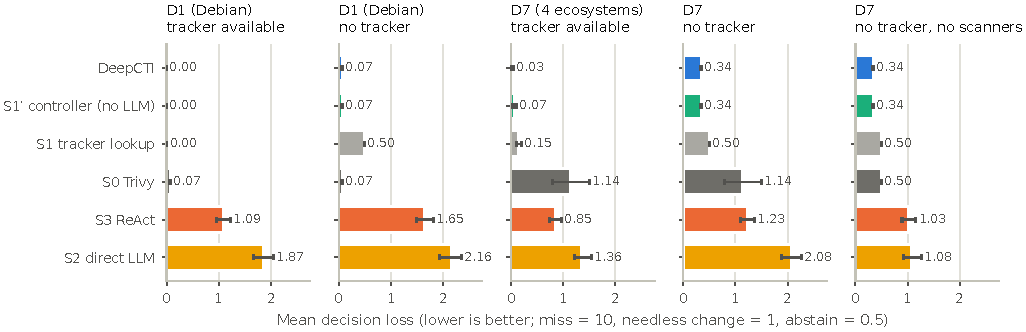
\includegraphics[width=\textwidth]{figs/fig_main_loss.pdf}
\caption{Mean decision loss on the test splits (pooled over models; whiskers: CVE-clustered 95\% CIs). With
a tracker, \DC{} matches a lookup. Without one, it decides from trusted sources (on D1, the trusted
scanners) and abstains where none decides (D7), whereas ReAct (S3) and direct prompting (S2) miss
vulnerabilities. Trivy is trusted on D1 but noisy on D7.}
\label{fig:main}
\end{figure*}

\begin{table}[t]
\caption{Pre-registered hypotheses (test split; estimate with 95\% CI). Loss and cost differences are
\DC{} minus comparator (negative favours \DC{}). Decision rules as pre-registered (\S\ref{sec:eval}).}
\label{tab:hyp}
\centering\scriptsize
\setlength{\tabcolsep}{2pt}
\begin{tabularx}{\columnwidth}{@{}lXrc@{}}
\toprule
& \textbf{Claim} & \textbf{Estimate} & \textbf{Held}\\
\midrule
\multicolumn{4}{@{}l}{\textit{prereg-v1: D1--D3, 6 models}}\\
H0 & tracker arm: DC $\equiv$ S1 accuracy ($\pm$3 pp) & +0.002 & yes\\
H1 & withheld: loss DC $<$ S3 & $-1.585$ [$-1.76,-1.42$] & yes\\
H2 & D2: staleness error DC $<$ S3 & $-0.264$ & yes\\
H3 & EC$^2$ cheaper than checklist & $-0.03$, $p{=}1$ & \textbf{no}\\
H4 & attack success DC+P3 $<$ S3+P1 & $-0.099$ & yes$^\dagger$\\
H5 & LTT risk $\le\alpha$ (withheld) & vacuous & --\\
\multicolumn{4}{@{}l}{\textit{prereg-v2: D1/D2, 9 models}}\\
H7 & upgrade w/o restart: DCv21 $<$ DC & $-9.25$ [$-9.76,-8.43$] & yes$^\ddagger$\\
H8 & other drift: DCv21 non-inferior & 0.000 & yes\\
\multicolumn{4}{@{}l}{\textit{prereg-v3: D7, 8 models (H14: 2; H15: 7 generators)}}\\
H9 & withheld: loss DC $<$ S3 & $-0.883$ [$-1.03,-0.74$] & yes\\
H10 & vendor, tracker: DC $<$ S1$'$ (LLM-free) & $-0.205$ [$-0.26,-0.14$] & yes\\
H11 & accepted-fact error DC $<$ noverify & $-0.027$ [$-0.04,-0.02$] & yes\\
H12 & LTT blind arm, $\alpha{=}0.05$ & $\ge$93\% splits & yes\\
H13 & D7 drift: DCv21 $<$ DC & $-4.59$ [$-6.30,-3.02$] & yes\\
H14 & EC$^2$ cheaper than checklist & $-0.35$ [$-0.51,-0.21$] & yes\\
H15 & DCv21 notes non-inferior ($-0.02$) & $-0.018$ [$-0.05,+0.01$] & \textbf{no}\\
\multicolumn{4}{@{}l}{\textit{prereg-v4: D7, 8 models}}\\
H16 & DCv21b notes non-inferior ($-0.02$) & $+0.044$ [$+0.01,+0.07$] & yes\\
H17 & DCt (more trust data) $<$ DC, withheld & $-0.137$ [$-0.17,-0.11$] & yes\\
H18 & decoys: DC loss non-inferior ($+0.05$) & $-0.026$ [$-0.05,-0.01$] & yes$^\S$\\
\bottomrule
\multicolumn{4}{@{}l}{\parbox{\columnwidth}{\tiny $^\dagger$attacks barely moved S3 (\S\ref{sec:sec}).
$^\ddagger$confirmatory only: these episodes motivated v2.1. $^\S$baseline ran on older code; same-code
control: $-0.001$ [$-0.002,0$], low exposure (\S\ref{sec:v4}). H6 (model-size interaction) exploratory.}}
\end{tabularx}
\end{table}

\subsection{Decisions without a feed}

Fig.~\ref{fig:main} and Table~\ref{tab:hyp} give the headline results. With a tracker, \DC{} has zero
loss on D1 and is equivalent to the lookup (H0). On D7, its loss is 0.030, compared with 0.071 for
S1$'$ and 0.147 for S1. Without a tracker, ReAct's loss rises to 1.65 (D1) and 1.23 (D7). Its errors are
mostly misses: DER is 0.49 on D1 and 0.30 on D7. \DC{}, by contrast, has DER 0 in every arm. On D7 its
coverage is 0.31: it abstains when no trusted source decides. H1 and H9 hold with large margins.

On D1 the result holds for every model (Fig.~\ref{fig:scale}). ReAct loss with a tracker ranges from
0.18 (Gemma-31B) to 2.64 (Qwen3-4B), and reliability under resampling (pass$^5$ at $T{=}0.7$) ranges from 0.98
(Gemma-31B) to 0.08 (Llama-8B), or 0.00 for Nemotron-49B; \DC{}'s pass$^5$ is 1.0 for all nine models. \DC{}'s decisions are identical for every model. On D7 there is
one exception: without a feed, Gemma-31B ReAct has lower loss than \DC{} (0.291 vs.\ 0.344, DER 0.047
vs.\ 0), and without scanners the two are about equal (0.365 vs.\ 0.344). ReAct trades misses for
coverage, \DC{} abstains. The largest model narrows but does not close the pooled gap: Mistral-Medium-128B ReAct exceeds \DC{} by 0.41 (D1 tracker), 0.79 (D1 withheld), 0.18
(D7 tracker) and 0.30 (D7 withheld). Inspect AI's ReAct agent agrees with ours on 80.6\% of D7 decisions
($n{=}1{,}635$). With a tracker its loss is similar (0.92/1.14 versus S3's 0.84/1.13 for
Mistral-24B/Qwen3-14B). Without one it is somewhat lower (1.50/1.51 versus 1.63/2.14), so our ReAct
baseline is, if anything, slightly weaker than a standard harness in that arm.

\begin{figure}[t]
\centering
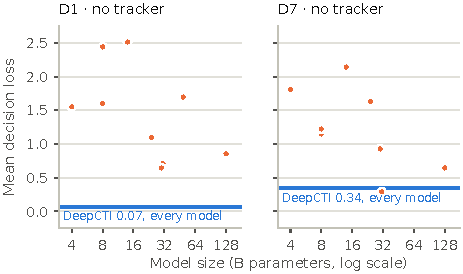
\includegraphics[width=\columnwidth]{figs/fig_scaling.pdf}
\caption{ReAct (S3) loss per model versus parameter count, no-tracker arms. Each dot is one model. The
blue line is \DC{}, whose decisions are identical for every model.}
\label{fig:scale}
\end{figure}

\subsection{What the language model contributes}

On D1, and in both feed-less D7 arms, \DC{}'s decisions equal those of the LLM-free controller S1$'$: the advantage comes from the evidence state and decision table, not from model reasoning. The LLM
matters in two places.

\textbf{Unstructured evidence.} For vendor software, the version exists only in text files (release notes,
headers, configuration files) and banners. There, in the tracker arm, verified extraction lowers loss relative to S1$'$ by 0.205 (H10). Verification
reduces the share of accepted version facts that are wrong by 2.7 percentage points (H11;
Fig.~\ref{fig:extract}). It rejects 9\% of proposals from files and 17\% from process banners, and it eliminates wrong facts
from banners (4.1\% to 0\%). On benign vendor cases with a tracker, unverified extraction nevertheless had lower loss (0.084
vs.\ 0.146). Most of that gap was a verifier bug: header banners such as \texttt{X-Jenkins:} were rejected.
With the bug fixed post hoc (a logged deviation; 8 models), the gap is 0.113 vs.\ 0.084.

\begin{figure}[t]
\centering
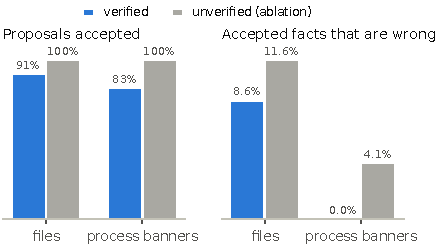
\includegraphics[width=\columnwidth]{figs/fig_extraction.pdf}
\caption{Verified versus unverified LLM extraction on D7 (all arms, 8 models): share of proposed
version facts admitted, and share of admitted facts that are wrong.}
\label{fig:extract}
\end{figure}

\textbf{Risk-controlled release.} In the blind arm, hints point to a decision for most abstentions. We pool calibration and test records and draw 200 CVE-level re-splits (40\% calibrate, 60\% evaluate).
LTT then raises coverage from 0.31 to between 0.50 (Qwen3-4B) and 0.91 (Mistral-Medium). Mean realised
risk is 1.4--1.9\%, and at least 93\% of re-splits stay within $\alpha$ for every model (H12;
Fig.~\ref{fig:ltt}). Here coverage scales with model quality while
the risk guarantee does not depend on it. This is the converse of ReAct, where quality and risk move together.

\begin{figure}[t]
\centering
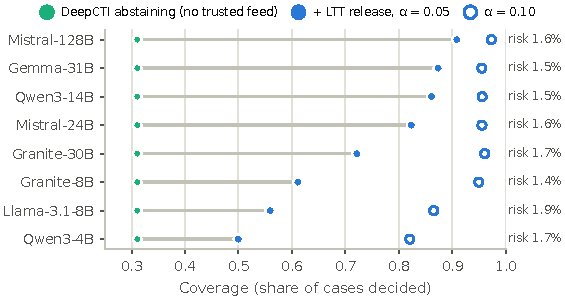
\includegraphics[width=\columnwidth]{figs/fig_ltt.pdf}
\caption{Learn-then-Test release of hint-based decisions, D7 blind arm. Coverage without release (green),
with release at $\alpha{=}0.05$ (filled) and $0.10$ (open); mean realised risk at $\alpha{=}0.05$
over 200 CVE re-splits on the right.}
\label{fig:ltt}
\end{figure}

\subsection{Drift}

On D2, \DC{} reports the pre-drift status when it is wrong less often than ReAct (H2). The first version,
however, was \emph{restart-blind} (Fig.~\ref{fig:drift}). When a package is upgraded without a restart,
package database, changelog and scanners all say \emph{fixed} while the vulnerable binary keeps running.
DC's loss on these episodes is 9.67 (accuracy 0), worse than ReAct under the original prompt (7.56).
For the v2.1 study all systems shared a revised prompt that tells them to check running services, and
ReAct's loss fell to 3.98. Instance-aware evidence
(DCv21) reduces the loss to 0.42 (accuracy 0.93, H7) and is non-inferior on all other D2 drift kinds (H8).
Because these episodes motivated the fix, we pre-registered an independent test on fresh D7 drift
episodes. There, DCv21 has loss 0.45, against 5.04 for DC and 2.03 for ReAct (H13). On rollbacks ReAct
fails (loss 4.08 on D7, 6.87 on D2), while both \DC{} versions stay near zero. The fix has a cost on D7. On upgrades \emph{with} restart DCv21 abstains more (accuracy 0.74 vs.\ 0.95,
loss 0.128 vs.\ 0.025). It also needs more tool cost: 8\% more in the main D7 study and 34--79\% more on
the drift episodes.

\begin{figure*}[t]
\centering
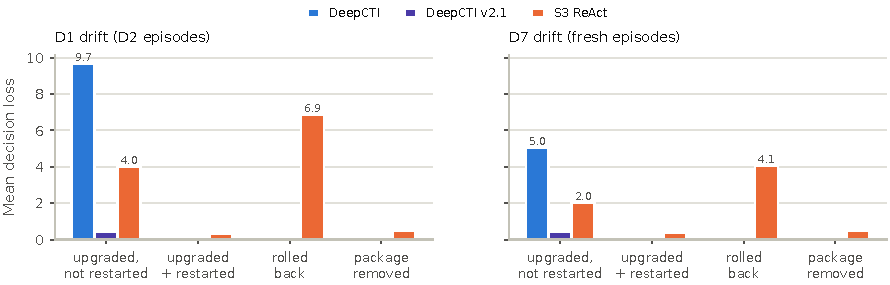
\includegraphics[width=\textwidth]{figs/fig_drift.pdf}
\caption{Decision loss by drift kind. Left: D2 (9 models). Right: fresh D7 drift episodes (8 models).
The original controller is restart-blind; instance-aware evidence (v2.1) removes the failure. It is
non-inferior on the other D2 kinds, but on D7 it abstains more after restarts.}
\label{fig:drift}
\end{figure*}

\subsection{Acquisition}

On D1, acquisition does not matter: with a tracker every strategy except random order decides in about two
calls, and H3
fails ($-0.03$, $p{=}1$). On D7 without a tracker, where acquisition is non-trivial, EC$^2$ reaches a
decision with lower cost than the fixed checklist ($-0.35$ cost units at identical loss, H14;
Fig.~\ref{fig:acq}). Entropy-greedy is cheaper still (4.20 vs.\ 5.34 units), so we do not claim that
EC$^2$ is the best rule, only that VOI beats a fixed order. ReAct spends a similar budget at three to
five times the loss.

\begin{figure}[t]
\centering
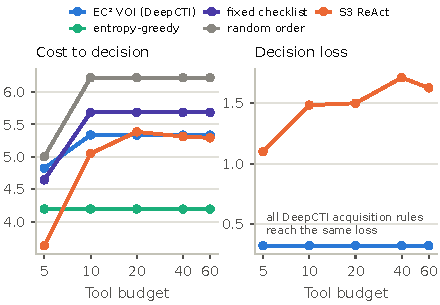
\includegraphics[width=\columnwidth]{figs/fig_acquisition.pdf}
\caption{Acquisition on D7, withheld arm (Qwen3-14B, Mistral-24B): mean tool cost to the decision and
decision loss by budget.}
\label{fig:acq}
\end{figure}

\subsection{Authorization}
\label{sec:sec}

On D3, an unmodified ReAct agent executes unauthorized disruptive actions in 5--6\% of episodes
(Fig.~\ref{fig:sec}). This happens without an attacker as well: the agent patches or restarts on its own
initiative. Argument checks (P1) and a prompt defence do not change the rate. Evidence gating (P3)
removes these actions for the same agent and for \DC{}. This has a liveness cost: ReAct+P3 blocked one
model's warranted remediations (false-block rate 0.33 over 6 warranted episodes). The $(k,m)$ grid
shows the guarantee's boundary:
\begin{itemize}
\item forging one trusted world group ($m{=}1<k{=}2$) yields no unauthorized action, while forging
  two ($m{=}k$) yields 0.017;
\item compromising the change system, whose atoms have $k{=}1$, yields 0.33 (6 episodes);
\item P3k3 ($k{=}3$) blocks all tested compromises.
\end{itemize}
The attack study is weak: injected text barely changed ReAct's behaviour (ASR minus the benign rate of
the same goal was $-0.005$). H4 therefore mostly measures ordinary errors, and we do not claim robustness
to adaptive injection.

\begin{figure}[t]
\centering
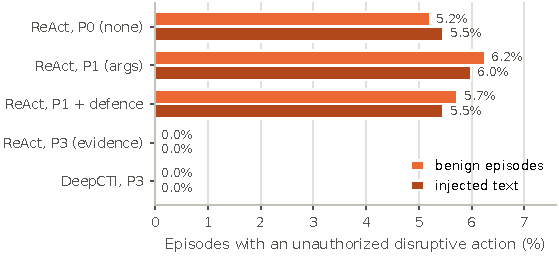
\includegraphics[width=\columnwidth]{figs/fig_security.pdf}
\caption{Episodes with an unauthorized disruptive action on D3 (3 models), benign versus injected
text. Evidence gating (P3) removes them; argument checks and a prompt defence do not.}
\label{fig:sec}
\end{figure}

\subsection{Analyst notes}
\label{sec:notes}

The v2.1 validator was pre-registered as non-inferior to DC's unvalidated notes (H15), and it failed
($-0.018$ [$-0.047,+0.010$]). The cause was a prompt defect: the synthesis prompt said ``the decision is
FIXED (do not change it)'', and 40.5\% of non-fixed notes then contained ``FIXED''. With a neutral prompt
(DCv21b, post hoc), faithfulness rose by $+0.036$ [$+0.011,+0.062$] over DC on the same sample, and
note--decision consistency was 0.978 (DC 0.960, DCv21 0.752). Of these notes, 90.9\% passed validation
on the first attempt, 3.4\% after repair, and 5.8\% fell back. We confirmed this on a fresh,
pre-registered sample of 504 triples drawn from cases disjoint from the H15 sample and covering all eight
generators (H16). DCv21b's faithfulness was 0.744 against DC's 0.700, a difference of $+0.044$
[$+0.014,+0.073$], so non-inferiority holds and the estimate excludes zero. Its note--decision
consistency was 0.988 (DC 0.961), and 6.0\% of its notes fell back to the deterministic template
(Fig.~\ref{fig:notes}).

\begin{figure}[t]
\centering
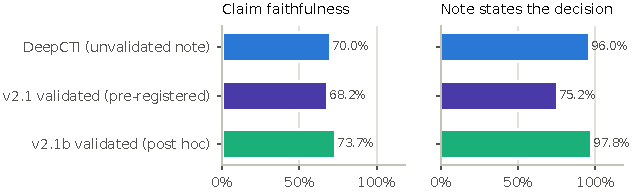
\includegraphics[width=\columnwidth]{figs/fig_notes.pdf}
\caption{Analyst-note quality (D7): share of atomic claims judged supported by up to three validated
judges from other model families, and share of notes stating the controller's decision.}
\label{fig:notes}
\end{figure}

\subsection{Trust estimation and decoys (prereg-v4)}
\label{sec:v4}

\textbf{Trust.} With trust estimated on 42 development CVEs, no scanner met the rule on D7, so DC
ignored scanners and abstained where scanners were right. Re-estimating on development plus calibration
data (71 CVEs) with the same rule trusts scanners for Ubuntu and Maven, but not for PyPI (false-negative
rate 10.5\%) or vendor software (where scanners never find the version). This DCt variant lowers withheld-arm loss
from 0.344 to 0.207 ($-0.137$ [$-0.167,-0.107$], H17) and raises coverage from 0.31 to 0.73, with DER
still 0. Its decisions are again identical across the eight models. Conservative trust was thus a
data-quantity problem, not a flaw of the rule.

\textbf{Decoys.} A realistic wrong version mention was added to the documents the systems actually read.
On vulnerable Ubuntu hosts it is a changelog body line naming the fixed version. In vendor software it is
a ``see also'' line in every document that states the installed version. A dev pilot showed that decoys
placed in unread notes are never observed. The pre-registered comparison passes ($-0.026$
[$-0.050,-0.006$], H18), but the audit found a confound. For seven models the clean baseline ran
before the verifier fixes, so that contrast mixes the decoy effect with a code change. We therefore
added a same-code control run without decoys (logged deviation). Against it, decoys change DC's loss by
$-0.001$ [$-0.002,0$], DC\_noverify's by 0, and ReAct's by $-0.02$ [$-0.13,+0.10$]. Neither DC nor DC\_noverify
ever accepted a decoy version as a fact. Exposure was low, however: DC read the decoy before deciding in only
11.5\% of episodes (3 CVEs), because it decides from the package database or tracker first. H18
therefore shows that such decoys are inert for \DC{}, not that its verifier would resist targeted
version spoofing.

\textbf{Panel completion.} On D3, Mistral-Medium-128B's ReAct agent took no unauthorized disruptive
action in benign episodes and 1.6\% under injected text, far fewer than the smaller models (5--6\%).
\DC{}+P3 stayed at 0\% in both conditions; under forged trusted groups its rates (3.1--4.7\%) equal
those of the other models, as the guarantee's boundary predicts. GLM-4.5-Air (106B MoE), added as a tenth model, reproduces the
pattern. Its ReAct loss is 0.97/1.48 on D1 (tracker/withheld) and 0.84/0.96 on D7, against \DC{}'s
0/0.07 and 0.02/0.34. On D7 upgrades without restart, its DCv21 loss is 0.025, against 5.06
for DC and 3.53 for ReAct.

%==============================================================================
\section{Discussion and Limitations}

\textbf{What carries the result.} The decisive ingredient is not the LLM but the evidence discipline:
\begin{itemize}
\item only trusted, independent, fresh observations change a decision;
\item missing or conflicting evidence yields an explained abstention;
\item disruptive actions need corroborated support.
\end{itemize}
This turns model quality from a safety variable into a coverage variable: under LTT, weaker models
release fewer decisions, but they do not miss more. The LLM earns its place where evidence is unstructured, through verified
extraction, and through risk-controlled release of hint-based decisions. An honest reading of H9 is
therefore ``evidence-state controller versus ReAct'', not ``better reasoning''.

\textbf{Costs.}
\begin{itemize}
\item Abstention costs coverage: 0.31 on D7 without a feed, before LTT.
\item Conservative trust discards useful sources when estimated on little data (repaired in H17).
\item Verification trades some benign-data coverage for precision.
\item Corroboration counts groups, not physical artefacts. With Maven scanners trusted (H17), a scanner
  and a direct jar read are distinct groups, although both read the same jar metadata.
\item Instance-awareness increases abstention after restarts and adds 34--140\% prompt tokens.
\item Transfer: on VEX-Bench (62 of 75 tasks), our evidence-state wrapper did not beat the benchmark's
  plain harness (status F1 0.613 vs.\ 0.648 with Gemma-31B; all paired CIs contain 0) and abstained on
  54--73\% of tasks.
\end{itemize}
Each of these costs is measured above, and none was tuned on test data.

\textbf{Threats to validity.}
\begin{itemize}
\item Tools are simulated over the fixtures. There were no containers, and no host software was
  executed; only the scanners ran on the file systems.
\item Labels come from trackers and advisories without a human audit; tracker lag and errors propagate
  into them.
\item Construction variants are label-correlated, but they are never shown to systems.
\item The attack study is weak (\S\ref{sec:sec}), and an adaptive-attack evaluation remains open.
\item Note quality is judged by LLMs, validated only by error injection.
\item Nemotron-49B's ReAct runs used a generic tool template, and 25.5\% of its D1 ReAct episodes made no
  tool call.
\item We did not run a practitioner study.
\end{itemize}

%==============================================================================
\section{Conclusion}

Mitigation decisions should be made by an explicit evidence state, not inside an LLM's context window.
\DC{} implements this with a provenance-tracked Belnap state, a VEX decision table, value-of-information
acquisition, verified extraction, risk-controlled release and evidence-conditioned authorization.
Across two live-fixture benchmarks, ten models and four pre-registered rounds, it avoids the missed
vulnerabilities that dominate LLM-agent loss in the main studies (drift remains harder). It confines the model to roles where it can be checked,
and it blocks unauthorized disruptive actions. The failures we found were a restart-blind controller,
conservative trust and a defective synthesis prompt. Each was diagnosed in the data, and each repair
was then tested on held-out data under a new pre-registration.

\bibliographystyle{IEEEtran}
\bibliography{deepcti_references}

\end{document}
